\documentclass[border=12pt]{standalone}
\def\pgfsysdriver{pgfsys-dvisvgm.def}
\usepackage[dvisvgm]{xcolor}
\usepackage{xeCJK}
\setCJKmainfont{HaranoAjiGothic-Regular.otf}[BoldFont=HaranoAjiGothic-Bold.otf]
\setCJKsansfont{HaranoAjiGothic-Regular.otf}[BoldFont=HaranoAjiGothic-Bold.otf]
\usepackage{amsmath,amssymb,tikz,lmodern}
\usetikzlibrary{arrows.meta,positioning,calc}
\renewcommand{\familydefault}{\sfdefault}
\definecolor{ink}{HTML}{25322F}
\definecolor{green}{HTML}{246657}
\definecolor{tint}{HTML}{EEF4F0}
\definecolor{soft}{HTML}{C6D2CC}
\definecolor{muted}{HTML}{52615B}
\newif\ifJapanese
\newcommand{\Tx}[2]{\ifJapanese #1\else #2\fi}
\newcommand{\heading}[3]{{\color{green}\bfseries #1\quad\Tx{#2}{#3}}\\[5pt]}
\newcommand{\Var}{\operatorname{Var}}
\newcommand{\Frac}{\operatorname{Frac}}
\newcommand{\C}{\mathbb C}
\newcommand{\refurl}[2]{\special{dvisvgm:raw <a xlink:href="#1" target="_blank" rel="noopener noreferrer">}{\setlength{\fboxsep}{0pt}\colorbox{white}{\color{green}\underline{\strut #2}}}\special{dvisvgm:raw </a>}}
\newcommand{\R}[2]{\refurl{\csname source#1\endcsname}{#2}}
\tikzset{
 card/.style={draw=soft,fill=white,rounded corners=2pt,align=left,text=ink,font=\fontsize{10.5}{14}\selectfont,inner xsep=12pt,inner ysep=11pt,text width=14.4cm},
 result/.style={card,draw=green,fill=tint,line width=.9pt},
 reason/.style={align=left,text=muted,font=\fontsize{9}{12}\selectfont,inner sep=0pt,text width=12.7cm},
 edge/.style={-{Stealth[length=2.4mm]},draw=green,line width=1pt}
}
\newcommand{\flow}[3]{
 \coordinate (#2-from) at ($(#1.south)+(-6.9,0)$);
 \coordinate (#2-to) at ($(#2.north)+(-6.9,0)$);
 \draw[edge] (#2-from)--(#2-to);
 \node[reason,anchor=west] at ($(#2-from)!.5!(#2-to)+(.55,0)$) {#3};
}

\Japanesefalse
\expandafter\def\csname sourceWV\endcsname{https://github.com/openai/math/blob/fd4aeeb2ee4fc729c18d98444fed42fd0529eeeb/preprints/Logarithmic-Kodaira-dimension-and-whole-fiber-variation-September-26-2026/paper.pdf}
\expandafter\def\csname sourceOI\endcsname{https://github.com/openai/math/blob/fd4aeeb2ee4fc729c18d98444fed42fd0529eeeb/preprints/Orbifold-and-logarithmic-Iitaka-subadditivity-September-26-2026/paper.pdf}
\expandafter\def\csname sourcePH\endcsname{https://github.com/openai/math/blob/fd4aeeb2ee4fc729c18d98444fed42fd0529eeeb/preprints/Projective-Hodge-lines-and-ordinary-Iitaka-subadditivity-September-27-2026/paper.pdf}
\expandafter\def\csname sourceRA\endcsname{https://github.com/openai/math/blob/fd4aeeb2ee4fc729c18d98444fed42fd0529eeeb/preprints/The-reverse-logarithmic-Kodaira-inequality-and-additivity-September-26-2026/paper.pdf}
\expandafter\def\csname sourceLA\endcsname{https://github.com/openai/math/blob/adc7f1241b42e322a6451854ab7e4b4c146bf78a/preprints/Log-abundance-in-characteristic-zero-September-24-2026/paper.pdf}
\expandafter\def\csname sourceFuj\endcsname{https://www.math.kyoto-u.ac.jp/~fujino/weak-posi11.pdf}
\expandafter\def\csname sourceDel\endcsname{https://www.numdam.org/item/PMIHES_1971__40__5_0.pdf}
\expandafter\def\csname sourceDHP\endcsname{https://arxiv.org/pdf/1012.0493v2}
\expandafter\def\csname sourcePT\endcsname{https://arxiv.org/pdf/1409.5504v1}
\expandafter\def\csname sourceBCHM\endcsname{https://arxiv.org/pdf/math/0610203v2}
\expandafter\def\csname sourceKP\endcsname{https://sites.math.washington.edu/~kovacs/2013/papers/Kovacs_Patakfalvi__Projectivity.pdf}
\expandafter\def\csname sourceHan\endcsname{https://doi.org/10.1007/BF01394338}
\expandafter\def\csname sourceSGA1\endcsname{https://arxiv.org/abs/math/0206203v2}
\expandafter\def\csname sourceLan\endcsname{https://arxiv.org/pdf/2005.09690v3}
\expandafter\def\csname sourceBDPP\endcsname{https://arxiv.org/pdf/math/0405285v1}
\expandafter\def\csname sourceTaj\endcsname{https://arxiv.org/pdf/2005.01025v4}
\begin{document}
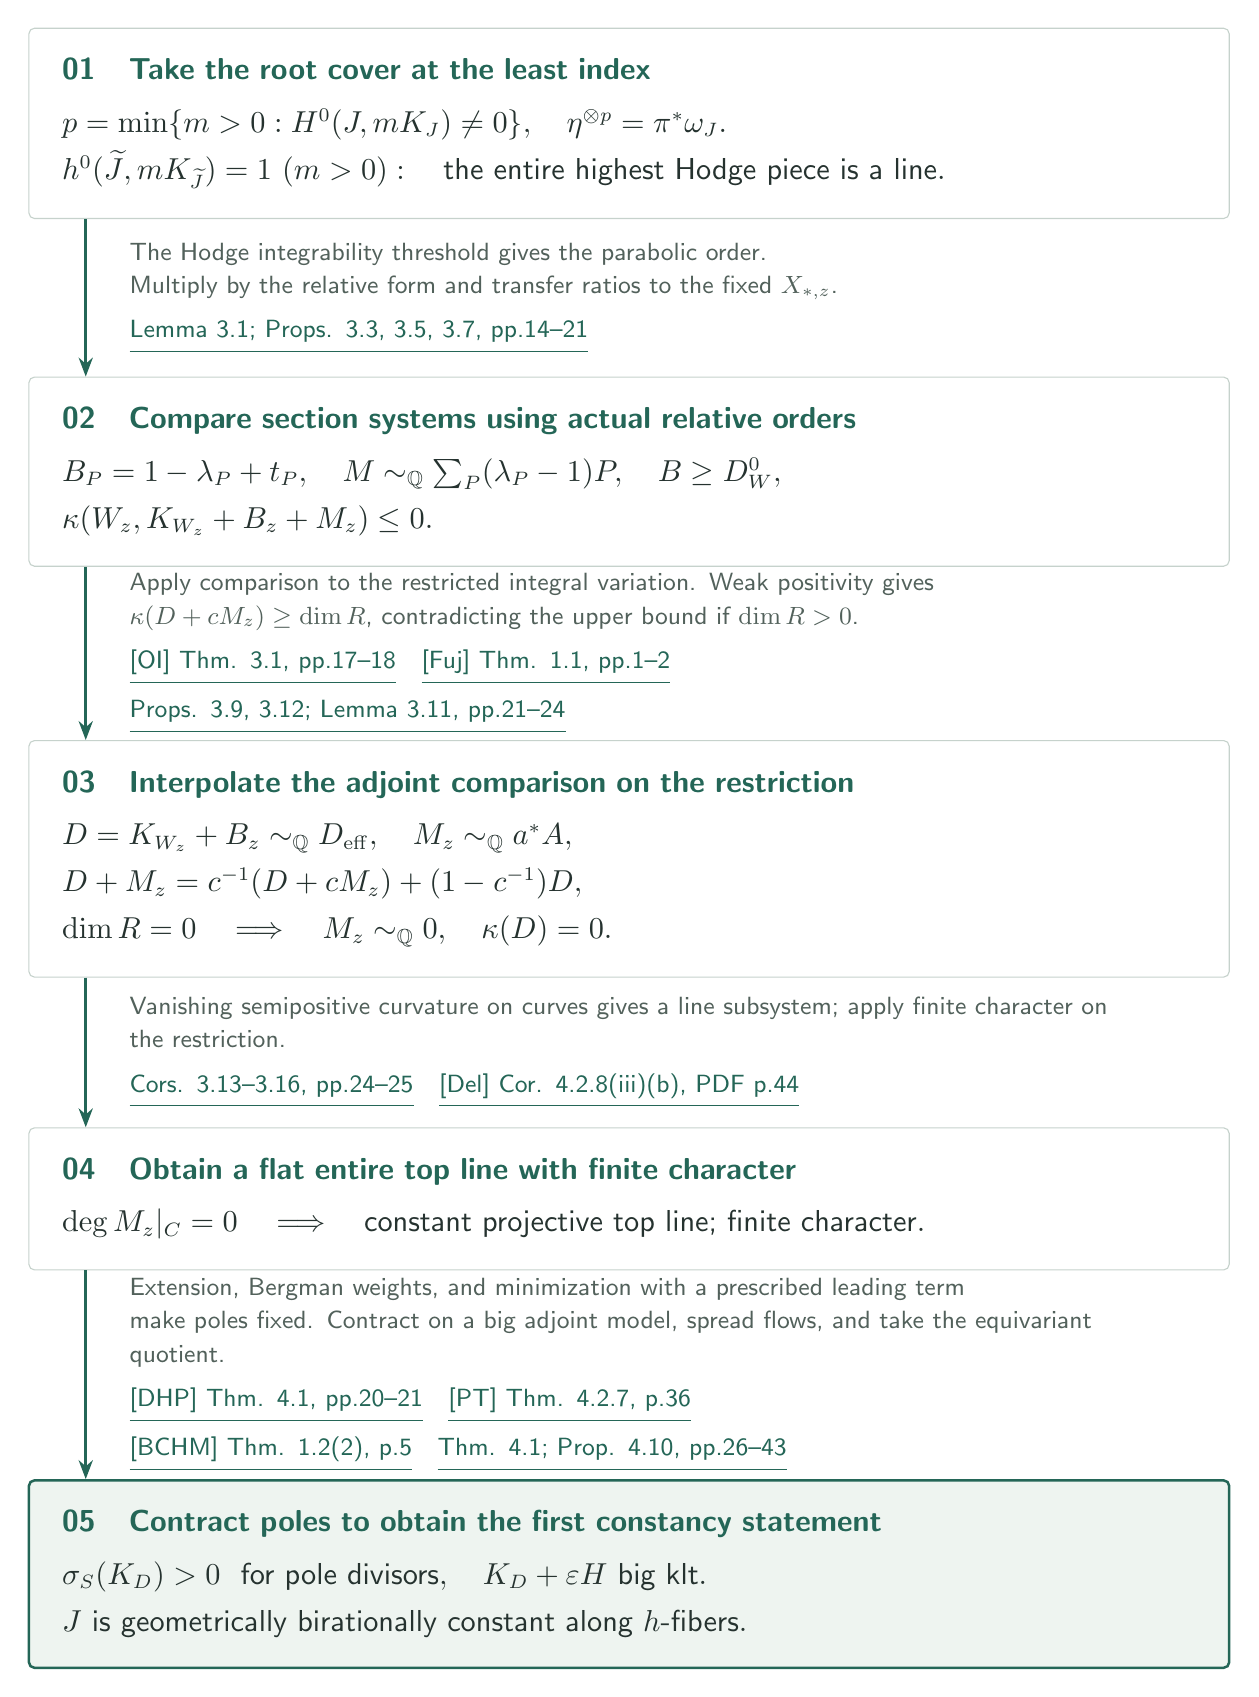
\begin{tikzpicture}
\node[card] (root) {\heading{01}{最小指数でroot coverを取る}{Take the root cover at the least index}
$p=\min\{m>0:H^0(J,mK_J)\ne0\},\quad \eta^{\otimes p}=\pi^*\omega_J.$\\[3pt]
$h^0(\widetilde J,mK_{\widetilde J})=1\ (m>0):\quad\Tx{\text{最高Hodge成分全体が直線}}{\text{the entire highest Hodge piece is a line}}.$};
\node[card,below=2cm of root] (bound) {\heading{02}{実際の位数で切断系を比較する}{Compare section systems using actual relative orders}
$B_P=1-\lambda_P+t_P,\quad M\sim_{\mathbb Q}\sum_P(\lambda_P-1)P,\quad B\ge D_W^0,$\\[3pt]
$\kappa(W_z,K_{W_z}+B_z+M_z)\le0.$};
\flow{root}{bound}{\Tx{Hodge normの可積分閾値がparabolic orderを与える。\\相対形式を掛け、固定された $X_{*,z}$ に切断比を移す。}{The Hodge integrability threshold gives the parabolic order.\\Multiply by the relative form and transfer ratios to the fixed $X_{*,z}$.}\\[4pt]
\R{WV}{Lemma 3.1; Props. 3.3, 3.5, 3.7, pp.14--21}}
\node[card,below=2.2cm of bound] (trivial) {\heading{03}{制限後の随伴比較を補間する}{Interpolate the adjoint comparison on the restriction}
$D=K_{W_z}+B_z\sim_{\mathbb Q}D_{\rm eff},\quad M_z\sim_{\mathbb Q}a^*A,$\\[3pt]
$D+M_z=c^{-1}(D+cM_z)+(1-c^{-1})D,$\\[3pt]
$\dim R=0\quad\Longrightarrow\quad M_z\sim_{\mathbb Q}0,\quad\kappa(D)=0.$};
\flow{bound}{trivial}{\Tx{制限したintegral variationに比較を適用。weak positivityから\\$\kappa(D+cM_z)\ge\dim R$ となり、$\dim R>0$ は上界と矛盾する。}{Apply comparison to the restricted integral variation. Weak positivity gives\\$\kappa(D+cM_z)\ge\dim R$, contradicting the upper bound if $\dim R>0$.}\\[4pt]
\R{OI}{[OI] Thm. 3.1, pp.17--18}\quad\R{Fuj}{[Fuj] Thm. 1.1, pp.1--2}\\[3pt]
\R{WV}{Props. 3.9, 3.12; Lemma 3.11, pp.21--24}}
\node[card,below=1.9cm of trivial] (flat) {\heading{04}{最高成分のflatnessと有限指標を得る}{Obtain a flat entire top line with finite character}
$\deg M_z|_C=0\quad\Longrightarrow\quad \Tx{\text{projective top lineが一定、指標は有限}}{\text{constant projective top line; finite character}}.$};
\flow{trivial}{flat}{\Tx{曲線上で半正曲率を消し、制限上のrank-one subsystemに有限指標定理を使う。}{Vanishing semipositive curvature on curves gives a line subsystem; apply finite character on the restriction.}\\[4pt]
\R{WV}{Cors. 3.13--3.16, pp.24--25}\quad\R{Del}{[Del] Cor. 4.2.8(iii)(b), PDF p.44}}
\node[result,below=2.65cm of flat] (constant) {\heading{05}{極を収縮して最初のconstancyを得る}{Contract poles to obtain the first constancy statement}
$\sigma_S(K_D)>0\ \Tx{\text{（極の因子）}}{\text{ for pole divisors}},\quad K_D+\varepsilon H\ \text{big klt}.$\\[3pt]
$J\ \Tx{\text{は }h\text{-fiber方向で幾何学的に双有理一定}}{\text{is geometrically birationally constant along }h\text{-fibers}}.$};
\flow{flat}{constant}{\Tx{拡張・Bergman weight・先頭係数を固定する最小化で極を固定成分にする。\\big adjoint modelで収縮し、flowを代数化する。巡回作用を保ち商を取る。}{Extension, Bergman weights, and minimization with a prescribed leading term\\make poles fixed. Contract on a big adjoint model, spread flows, and take the equivariant quotient.}\\[4pt]
\R{DHP}{[DHP] Thm. 4.1, pp.20--21}\quad\R{PT}{[PT] Thm. 4.2.7, p.36}\\[3pt]
\R{BCHM}{[BCHM] Thm. 1.2(2), p.5}\quad\R{WV}{Thm. 4.1; Prop. 4.10, pp.26--43}}
\end{tikzpicture}

\end{document}
